\documentclass{pracamgr}

\usepackage{polski}

\usepackage[utf8]{inputenc}
\usepackage[T1]{fontenc}
\usepackage{algorithm}
\usepackage[noend]{algpseudocode}
\usepackage{amsmath}
\usepackage{graphicx}
\usepackage{tikz}
\usepackage{verbatim}
\usepackage{enumitem}
\usepackage[title,titletoc]{appendix}
\usepackage[labelfont=bf]{caption}
\usepackage{float}

\floatstyle{boxed}
\newfloat{algorytm}{h}{}
\floatname{algorytm}{Algorytm}

\floatstyle{plain}
\newfloat{rysunek}{h}{}
\floatname{rysunek}{Rysunek}


% version header
\usepackage{fancyhdr}
\pagestyle{fancy}
\fancyhead{}
\fancyhead[C]{wersja 2}

\fancypagestyle{plain}{%
}
\fancypagestyle{empty}{%
}
%%% version head


\usetikzlibrary{arrows}

\graphicspath{{img/}}

\author{Bartosz Marcinkowski}

\nralbumu{319476}

\title{Sztuczna inteligencja dla gry Quoridor}
\tytulang{Artificial intelligence for the Quoridor game}

\kierunek{Informatyka}

\opiekun{prof. Jana Madeya}

\date{Maj 2017}

\dziedzina{11.3 Informatyka}

\klasyfikacja{
I. Computing Methodologies \\
  I.2. Artificial intelligence \\
  I.2.1. Applications and Expert Systems}

\keywords{
	sztuczna inteligencja, gry planszowe, minimax
}

% Tu jest dobre miejsce na Twoje własne makra i~środowiska:
\newtheorem{defi}{Definicja}[section]

% koniec definicji

\begin{document}
\maketitle

\begin{abstract}
W pracy dokonujemy przeglądu algorytmów sztucznej inteligencji dla gier planszowych i opisujemy ich wykorzystanie na potrzeby aplikacji grającej w Quoridor.
\end{abstract}

\tableofcontents
%\listoffigures
%\listoftables


\chapter{Wprowadzenie}

\section{Tematyka pracy}

W pracy zajmiemy się algorytmami sztucznej inteligencji na potrzeby wytwarzanego oprogramowania --- komputerowej wersji gry planszowej Quoridor.
Aplikacja ta będzie umożliwiać wybór algorytmu sterującego każdym z uczestników gry albo pozostawienie tej roli samemu użytkownikowi.
Opiszemy powszechnie stosowane podejścia do problematyki oraz nasze próby ich wykorzystania.
Spróbujemy ocenić efekty swojej pracy i wyciągnąć wnioski przydatne w dalszej pracy nad sztuczną inteligencją w tej lub podobnych aplikacjach.

\section{Quoridor --- oryginalne zasady gry}

Gra rozgrywa się na planszy za pomocą 4 pionków i 20 ogrodzeń, nazywanych też \emph{ścianami}. Na planszy znajduje się siatka szczelin wyznaczająca 81 kwadratowych pól, tworzących układ 9~x~9. Każdy pionek ma unikatowy kolor, mieści się na jednym polu planszy i nie może go dzielić z innym. Ogrodzenia są identyczne i dają się umieszczać w szczelinach między polami planszy. Ogrodzenie jest dwukrotnie dłuższe od boku pola, więc (poprawnie umieszczone) sąsiaduje z dwoma polami z każdej strony, zajmuje całą szerokość szczeliny i jedno skrzyżowanie szczelin.

W grze może wziąć udział dwóch lub czterech graczy. W obu przypadkach otrzymują po jednym pionku, dzielą się po równo ogrodzeniami i przypisują się do różnych boków planszy; jeżeli jest ich dwóch, muszą to być boki przeciwległe.

Na początku gry na planszy nie ma ogrodzeń (stanowią zasoby graczy), a pionek każdego gracza umieszcza się na polu przy środku boku, do którego jest przypisany.
Następnie gracze wykonują kolejno swoje ruchy. Celem gry jest dotarcie swoim pionkiem do boku planszy przeciwległego wobec boku, do którego jest się przypisanym. Gra kończy się w momencie, w którym jednemu z graczy się to uda.

Każdy ruch może polegać na ustawieniu jednego ze swoich nieużytych ogrodzeń na planszy albo przesunięciu pionka. Ogrodzenie nie może kolidować z żadnym innym i nie może odciąć żadnemu graczowi wszystkich dróg do celu. Ruch pionkiem polega na przesunięciu go na puste, sąsiadnie pole (sąsiedztwo wyznacza wspólny bok).

Jeżeli na pewnym sąsiednim, nieodgrodzonym polu znajduje się już pionek przeciwnika, można wykonać skok na pole za tym pionkiem, o ile jest ono puste i nieodgrodzone. Jeżeli taki skok nie jest możliwy, można wykonać skok na jedno z dwóch pozostałych pól sąsiadujących z przeciwnikiem, znów o ile jest puste i nieodgrodzone.

\section{Cele i założenia}

Opracowywanie sztucznej inteligencji do gier planszowych może mieć różne założenia i cele.
Pełne rozwiązanie gier z dużą liczbą stanów wymaga mocy obliczeniowej przekraczającej możliwości komputera osobistego, a nawet jeśli uzyska się je na superkomputerze, to wynikowa tablica optymalnych ruchów nie nadaje się do dystrybucji wraz z grą.
Celem tej pracy jest opracowanie algorytmów sztucznej inteligencji dla gry Quoridor i utworzenie prototypu oprogramowania otwartoźródłowego, łatwego w dystrybucji i nadającego się do użycia na komputerze osobistym lub urządzeniu przenośnym, które będzie umożliwało grę w obu wariantach gry (dla 2 i 4 graczy), przy czy każdy gracz może być człowiekiem albo graczem komputerowym sterowanym przez jeden z dostępnych algorytmów sztucznej inteligencji.

\section{Istniejące rozwiązania}

Dostępnych jest już kilka programów grających w Quoridor. Są to aplikacje działające w przeglądarce internetowej. Żadna z nich nie osiąga celów, jakie postawiliśmy tworzonemu przez nas oprogramowaniu.
Tylko w jednym przypadku\footnote{http://danielborowski.com/quoridor-ai/v2/display.html} udostępniony jest kod źródłowy.
Inna aplikacja\footnote{https://play.google.com/store/apps/details?id=com.codestare.corridor}, wciąż w trakcie rozwoju, jest jedyną implementująca oba warianty gry.

\section{Struktura pracy}

W drugim rozdziale określimy szerszą klasę gier, w której znajduje się Quoridor.
Wprowadzimy pojęcia używane do ich opisu i algorytmy sztucznej inteligencji, które są wobec nich standardowo stosowane.

W trzecim rozdziale określimy te aspekty aplikacji, którę są istotne dla graczy komputerowych (dalej ,,botów'').
Tak więc doprecyzujemy zasady gry, wybierzemy technologie, zdefiniujemy interfejs bota, ograniczenia wykorzystania zasobów i oczekiwany czas działania.

W czwartym rozdziale opiszemy proces rozwijania kolejnych algorytmów.
Uzasadnimy wybór tych, które zaimplementujemy, wymienimy napotykane problemy oraz przedstawimy nasze rozwiązania.

W piątym rozdziale podsumujemy efekty naszej pracy.
Wskażemy kierunki dalszego ulepszania stworzonych botów i spróbujemy wyciągnąć wnioski przydatne przy implentacji komputerowych wersji innych gier.

\chapter{Standardowe metody dla stosownej klasy gier}

\section{Klasyfikacja Quoridor}

Żeby poznać stan wiedzy na temat sztucznej inteligencji w grach takich jak Quoridor, musimy najpierw określić tę klasę gier.
Cechy gry mające decydujący wpływ na algorytmy sterujące botami to:

 - podział na tury lub ciągłe wykonywanie ruchów,

 - pełna lub niepełna informacja o stanie gry,

 - istnienie elementów losowości,

 - podział zysku,

 - liczba graczy.

Na wyjaśnienie zasługuje tu ,,podział zysku''.
Ta cecha gry określa sposób, w jaki gracze są nagradzani, w szczególności decyduje o tym, czy jest opłacalna kooperacja. I tak na przykład szachy, są grą o sumie stałej, tzn. korzyść przeciwnika jest jednoznaczna ze stratą. Inaczej bywa w grach ekonomicznych, gdzie współpraca między graczami może zwiększyć wypłatę nagrody dla obu graczy.

Quoridor jest grą z podziałem na tury, z pełną informacją o stanie gry, bez losowości i jest grą o sumie stałej.
A więc w wariancie dla dwóch graczy znajduje się w tej samej klasie gier co szachy, warcaby, go i wiele innych klasycznych gier, którymi informatyka zajmuje się od dziesięcioleci.
Wiele z metod dla tej klasy gier zasłużyło już na miano standardowych.

Wariant dla czterech graczy wciąż pozostaje pod wieloma względami podobny do gier klasycznych.
Nie ma osobnego zestawu standardowych metod dla tego przypadku, który moglibyśmy tu przedstawić.
Stosuje się, o ile to możliwe, specjalne warianty algorytmów używanych dla dwóch graczy.

Od tej pory będziemy mówić wyłącznie o grach o sumie zerowej, z pełną informacją o stanie gry, w których gracze wykonują ruchy na zmianę.
Po wprowadzeniu podstawowych pojęć, zaprezentujemy metody standardowe (na podstawie~\cite{pawlewicz}), napierw specyficzne dla gier dwuosobowych (Minimax i Alfa-Beta), później niezależne od liczby graczy (Monte Carlo).
Na końcu przestawimy metody dostosowania algorytmów typowych dla gier dwuosobowych do gier z większą liczbą graczy.

\section{Podstawowe pojęcia}

Podstawową abstrakcją używaną do opisu gry jest graf skierowany, w którym wierzchołki reprezentują stany gry, a krawędzie odpowiadają legalnym ruchom.
Rozgrywka jest ścieżką, być może zawierającą cykle, od stanu początkowego do jednego ze stanów końcowych.

Na potrzeby algorytmów sztucznej inteligencji często wygodniej jest użyć drzewa gry, w którym wielu wierzchołkom może odpowiadać ten sam stan gry.
Stan, dla którego ma być wybrany kolejny ruch, jest reprezentowany przez korzeń, stany końcowe przez liście, a możliwy dalszy przbieg rozgrywki przez ścieżkę od korzenia do liścia.

W dalszej części pracy będziemy zamiennie używać pojęć stan i wierzchołek, ruch i krawędź itd. o ile nie będzie powodować to nieporozumień.

Kolejnym pojęciem pojawiającym się w tych algorytmach jest funkcja oceniająca.
Jest to funkcja przypisująca stanowi gry liczbę całkowitą, która ma oceniać jak bardzo pożądany jest ten stan dla danego gracza.
Powinna przyjmować skrajne wartości dla stanów końcowych (największą dla wygrywających, a najmniejszą dla przegrywających).

\section{Minimax i Alfa-Beta}

Algorytmy Minimax i Alfa-Beta zostały zaprojektowany z myślą o grach dwuosobowych.
W grze dwuosobowej o sumie zerowej przyjmujemy, że dla każdego stanu funkcja oceniająca jednego gracza przyjmie wartość przeciwną do funkcji oceniającej drugiego gracza.
A więc można wybrać jedną z tych funkcji oceniających jako jedyną interesującą.
Gracz, którego funkcja została wyróżniona nazywany jest wtedy \(max\), a jego przeciwnik \(min\).
Zgodnie z intuicją, gracz \(max\) wybiera stany maksymalizujące wartość wyróżnionej funkcji, a gracz \(min\) minimalizujące.

\subsection{Minimax}

Algorytm Minimax rozpatruje w drzewie gry tylko poddrzewo bieżącego stanu gry do ustalonej głębokości. W tak uzyskanym drzewie, liściom jest przypisana wartość funkcji oceniającej.
Pozostałe wierzchołki będą miały przypisywane wartości na podstawie wartości synów (patrz Algorytm \ref{minimax}).

\begin{algorytm}
\caption{Minimax\label{minimax}}
\begin{algorithmic}[1]
\Function{minimax}{$v$}
\If {$\texttt{\(v\) jest liściem}$}
	\State \Return $funkcjaOceniajaca(v)$
\EndIf
\If {$\texttt{ruch wykonuje gracz \(max\)}$}
    \State \Return $max$($minimax(w) | \texttt{\(w\) jest synem \(v\)})$
\Else
    \State \Return $min$($minimax(w) | \texttt{\(w\) jest synem \(v\)})$
\EndIf
\EndFunction
\end{algorithmic}
\end{algorytm}

Znając wartości \(minimax\) dla synów korzenia, możemy wybrać najkorzystniejszy ruch dla obecnego gracza.

\subsection{Alfa-Beta}

Algorytm Alfa-Beta jest ulepszeniem algorytmu minimax.
Opiera się na następującej obserwacji: wartości \(minimax\) niektórych wierzchołków mogą być ustalone bez obliczania ich dla wszystkich potomków aż do liści, a więc niektóre poddrzewa mogą zostać ,,odcięte'' (przykład na Rysunku \ref{alfa-beta-cut}).
Oszczędzając w ten sposób czas można zwiększyć głębokość przeszukiwanego drzewa, a więc podjąć lepszą decyzję.

\begin{rysunek}
\caption{Odcięcie w algorytmie Alfa-Beta \label{alfa-beta-cut}}
\centering
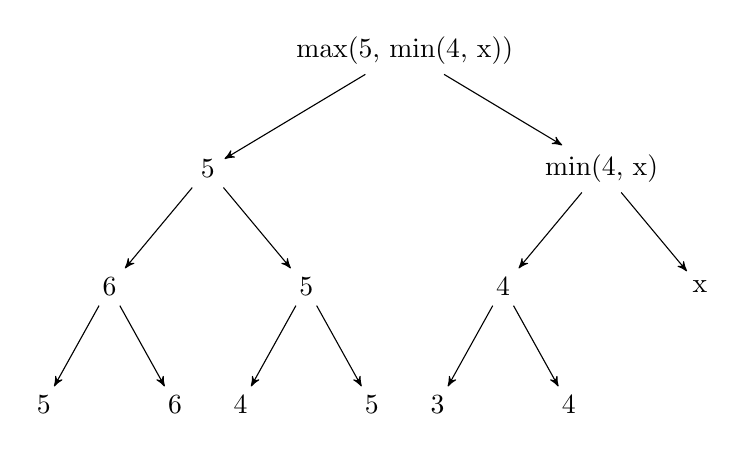
\begin{tikzpicture}[->,>=stealth',level/.style={sibling distance = 5cm/#1,
  level distance = 1.5cm}]
\node {max(5, min(4, x))}
    child{ node {5}
    	child{ node {6}
            child{ node {5}}
            child{ node {6}}
        }
		child{ node {5}
            child{ node {4}}
            child{ node {5}}
        }
    }
    child{ node {min(4, x)}
        child{ node {4}
            child{ node {3}}
            child{ node {4}}
        }
        child{ node {x}}
    }
;
\end{tikzpicture}

\end{rysunek}

Algorytm Alfa-Beta wprowadza pomocniczą funkcję \(alfabeta\):

\[
  \begin{cases}
    alfabeta(v, alfa, beta) \leq alfa    & \quad \text{if } minmax(v) \leq alfa\\
    alfabeta(v, alfa, beta) = minimax(v) & \quad \text{if } alfa < minmax(v) < beta \\
    alfabeta(v, alfa, beta) \geq beta    & \quad \text{if } minmax(v) \geq beta \\
  \end{cases}
\]

Przedział \((alfa, beta)\) jest nazywany \emph{oknem przeszukiwania} --- wartość wewnątrz niego to dokładnie obliczona wartosć \(minimax\).
Dla korzenia za okno przeszukiwania przyjmuje się przedział \((-\infty, \infty)\), a więc oblicza się dokładną wartość \(minimax\).
Znaczenie okna przeszukiwania można wyrazić następującą intuicją: jeżeli wartość obliczana dla danego wierzchołka jest większa niż \(beta\), to końcowy wynik obliczeń nie zmieni się, jeżeli za wartość bieżącego wierzchołka przyjmiemy \(beta\) lub dowolną większą liczbę; gracz \(min\) nie dopuści do rozpatrywanego stanu, ponieważ ma lepszą alternatywę.
Analogicznie, gdy wartość jest mniejsza niż \(alfa\), dla gracza \(max\) (patrz Algorytm \ref{alfabeta}).

\begin{algorytm}
\caption{Alfa-Beta\label{alfabeta}}
\begin{algorithmic}[1]
\Function{alfabeta}{$v, alfa, beta$}
\If {$\texttt{\(v\) jest liściem}$}
	\State \Return $funkcjaOceniajaca(v)$
\EndIf
    \If {\texttt{ruch wykonuje gracz \(max\)}}
    \ForAll {\texttt{\(w\) jest synem \(v\)}}
        \State $alfa \gets max(alfa, alfabeta(w, alfa, beta))$
        \If {$ alfa \geq beta$}
            \State \textbf{break}
        \EndIf
    \EndFor
	\State \Return $alfa$
\Else
    \ForAll {\texttt{\(w\) jest synem \(v\)}}
        \State $beta \gets min(beta, alfabeta(w, alfa, beta))$
        \If {$ alfa \geq beta$}
            \State \textbf{break}
        \EndIf
    \EndFor
	\State \Return $beta$
\EndIf
\EndFunction
\end{algorithmic}
\end{algorytm}

\subsection{Tablica transpozycji}

Ponieważ algorytmy Minimax i Alfa-Beta traktują graf gry jako drzewo, ten sam wierzchołek może być odwiedzony kilkukronie, o ile prowadzą do niego różne ścieżki.
Ta obserwacja jest podstawą techniki tablicy transpozycji, która pozwala na wykorzystanie wyników wcześniejszych obliczeń w trakcie działania algorytmu i przyspieszenie, dzięki któremu można zwiększyć głębokość przeszukiwania.

Zastosowanie tablicy transpozycji wymaga użycia funkcji haszującej \(h\), która umożliwi przypisanie każdemu stanowi gry liczbę całkowitą, ograniczoną z góry przez ustaloną wartość.
Należy też ustalić wielkość tablicy \(R\), która będzie musiała zmieścić się w pamięci dostępnej botowi.
Wtedy, po obliczeniu wartości wierzchołka \(w\), pod indeksem \(h(w)\ \textrm{mod}\ R\) tablicy haszującej umieszcza się wpis zawierający \(h(w)\), odległość wierzhołka \(w\) od korzenia w przeszukiwanym drzewie (wysokość) oraz specyficzne dla algorytmu wartości przydatne przy ponownym odwiedzeniu wierzchołka \(w\).
Zapisana wartość \(h(w)\), podczas odwiedzania wierzchołka \(v\) takiego, że \(h(w) \equiv h(v) (\textrm{mod}\ R)\), pozwala rozpoznać kolizję.
Zapisana wysokość wierzchołka \(w\) określa jakość wpisu.
Wysokość równa głębokości przeszukiwania oznacza, że wierzchołek był odwiedzony jako liść i zapisana wartość jest wprost wartością funkcji oceniającej dla tego wierzchołka.
Taką wartość uznajemy za gorszą od obliczonej dla wysokości o jeden mniejszej, kiedy rozpatrzone zostały wszystkie możliwe kolejne ruchy.
A zatem odnaleziony w tablicy transpozycji wpis może zostać użyty tylko wtedy, gdy zgadzają się wartości funkcji haszującej oraz wysokość zapisana we wpisie jest nie większa niż bieżąca.

W przypadku algorymu Minimimax dodatkowym polem wpisu jest to po prostu obliczona wartość wierzchołka, która może zostać użyta po spełnieniu wcześniej wymienionych warunków.

W przypadku algorytmu Alfa-Beta, wpis zawiera ograniczenie dolne i górne na wartość \(minimaks\) wierzchołka (równe sobie, jeżeli znana jest dokładna wartość).
Taki wpis nie zawsze pozwala natychmiast podać wynik, ale może zawęzić okno przeszukiwania i skrócić czas działania algorytmu.

\subsection{Inne ulepszenia}

Istnieją dalsze ulepszenia algorytmu Alfa-Beta (NegaScout, MTD-f), które opierają się na zawężaniu okna przeszukiwania.
Ten zabieg skraca czas działania, ale może nie dać przydatnego wyniku.
Na przykład, zamiast obliczać wartość \(alfabeta(w, alfa, beta)\) oblicza się \(alfabeta(w, alfa, beta')\), gdzie \(alfa < beta' < beta\).
Otrzymana wartość jest poprawnym wynikiem \(alfabeta(w, alfa, beta)\), o ile jest mniejsza od \(beta'\).
Choć obliczanie nieużytecznych wyników spowalnia algorytm, powinno zdarzać się rzadko.
Ostatecznie, skuteczność tych technik sprawdza się eksperymentalnie.

\section{Metody Monte Carlo}

Metoda Monte Carlo nie opiera się w żaden sposób na Minimax i w ogóle nie wymaga użycia funkcji oceniającej wartość wierzchołka.
Do jej zastosowania wystarczy znajomość zasad gry, to znaczy możliwych ruchów dla każdego stanu oraz stanów końcowych wraz z wynikiem rozgrywki.
Ruchy są oceniane na podstawie wyników losowych symulacji; w najprostszym algorytmie, od synów danego wierzchołka moglibyśmy rozpocząć równą liczbę losowych rozgrywek i wybrać tego, który najczęściej doprowadził do zwycięstwa.

\subsection{Monte Carlo Tree Search}

W praktyce prosta metoda Monte Carlo nie sprawdza się i należy w trakcie przeprowadzania symulacji niektóre wierzchołki początkowe porzucać jako mało obiecujące, a inne rozwijać, tzn. w ich miejsce wstawić wszystkich synów jako samodzielne wierzchołki początkowe symulacji.
Tak działa Monte Carlo Tree Search.

Algorytm ten utrzymuje drzewo, zakorzenione w wierzchołku dla którego wybiera ruch i początkowo posiadające ponad to wyłącznie liść dla każdego możliwego kolejnego stanu gry.
Każdy wierzchołek tego drzewa utrzymuje statystyki symulacji: liczbę symulacji i liczbę symulacji zakończonych zwycięstwem, które rozpoczęły się w poddrzewie danego wierzchołka.
Tak długo jak pozwalają na to limity czasu i pamięci, algorytm przechodzi od korzenia do pewnego liścia wybierając zawsze najbardziej obiecującego syna w zależności od wcześniej zebranych statystyk. Na podstawie statystyk liścia podejmuje decyzję o rozwinięciu go (dodaniu możliwych kolejnych stanów gry do drzewa ze statystykami) i jeśli to zrobi, wybiera jednego z dodanych synów, aby ostatecznie zawsze wybrać liść.
Dalej rozpoczyna od liścia losową rozgrywkę aż do poznania zwycięzcy, po czym aktualizuje statystyki wierzchołków na ścieżce od korzenia do liścia, z którego rozpoczęła się symulacja.
Najlepszy ruch z korzenia wyznacza jego syn, w którego statystykach stosunek zwycięstw do przeprowadzonych symulacji jest najkorzystniejszy.

W opisie algorytmu widać pewne luki: sposób wybierania najbardziej obiecującego syna i kryteria decyzji o rozwinięciu liścia.

Przy wybieraniu nabardziej obiecującego syna używa się metody granicy ufności.
Ma ona zapobiec sytuacji, w której po niewielkiej liczbie symulacji (nawet tylko jednej) liść jest porzucany, co ma miejsce gdy porównuje się wyłącznie stosunek liczby zwycięstw do liczby symulacji.
W tym celu to tego ilorazu jest dodawany \emph{współczynnik ufności}, tym wyższy im mniejszą częścią symulacji rodzica są symulacje danego syna. Jako współczynnik ufności przymuje się \(\sqrt{\frac{\sqrt{n_p}}{n_s}}\) lub \(\sqrt{\frac{\log{n_p}}{n_s}}\), gdzie \(n_s\) to liczba symulacji w poddrzewie syna, a \(n_p\) to liczba symulacji w poddrzewie rodzica.

Decyzję o rozwinięciu liścia podejmuje się na podstawie liczby symulacji, jakie zostały z niego rozpoczęte. Jeżeli przekroczy ustalony próg, zwykle zbliżony do liczby ruchów możliwych w jednym stanie gry, liść zostaje rozwinięty.

Oba parametry, tzn. wariant granicy ufności i próg rozwinięcia liścia, ustala się eksperymentalnie.

\section{Minimax dla wielu graczy}

Próby zastosowania algorytmu Minmax do gier wieloosobowych zostały podjęte na dwa sposoby.
Pierwszym było sprowadzenie gry wielosobowej do gry dwuosobowej, czego efektem jest algorytm Paranoid.
Drugim było osłabienie założeń i uogólnienie, czego efektem jest algorytm Max\textsuperscript{n}.
W przypadku obu algorytmów, zastosowanie dla dwóch graczy daje algorytm Minimax.

\subsection{Paranoid}

Redukcja gry wieloosobowej do gry dwuosobowej, jaka stoi za algorytmem Paranoid, jest następująca: gracz realizujący algorytm uznaje, że wszyscy przeciwnicy są w zmowie i jest im obojętne który z nich wygra.
Zależy im jedynie na zminimalizowaniu wyniku wyłączonego ze zmowy gracza.
Dzięki temu wszystkich przeciwników można traktować zbiorczo jako jednego i, zgodnie z założeniami Minimax, minimalizuje on wartości tej samej funkcji, którą gracz maksymalizuje.
Fakt, że ten zbiorczy przeciwnik może wykonywać więcej niż jeden ruch z rzędu i w jednym ruchu używa innego pionka niż w drugim, nie wpływa w żaden sposób na algorytm Minimax.

Redukcja do dwuosobowego algorytmu Minimax pozwala zastosować wprost wszystkie ulepszenia, jakie dla niego opracowano.
Niestety, zastosowane uproszczenie prowadzi do niekorzystnych decyzji, jeżeli przeciwnicy wcale nie są w zmowie (por. \cite{sturtevant}).

\subsection{Max\textsuperscript{n}}

Algorytm Max\textsuperscript{n} porzuca próby przypisywania każdemu stanowi pojedynczej liczby i zastępuje ją wektorem, w którym każdemu graczowi odpowiada dokładnie jedna liczba pod ustalonym inseksem.
Dla liści wektor jest tworzony przez obliczenie wartości funkcji oceniającej; wartość tej funkcji dla wybranego gracza znajdzie się pod przypisanym mu indeksem.
Wartością dla każdego innego wierzchołka jest ten wektor spośród wektorów-wartości jego synów, który ma największą wartość pod indeksem gracza wykonującego ruch.

Ten algorytm nie popełnia błędu algorymu Paranoid i zakłada, że każdy gracz próbuje zmaksymalizować własne szanse na zwycięstwo.
Niestety, nie da się wobec niego zastosować wprost ulepszeń Minimaksa, tzn. Alfy-Bety i manipulowania oknem przeszukiwań.

\subsection*{Ulepszenie Alfa-Beta dla algorytmu Max\textsuperscript{n}}

Da się jednak zastosować wobec algorytmu Max\textsuperscript{n} ulepszenie analogiczne do Alfy-Bety wobec Minimaksa (por. \cite{korf}), o ile dysponuje się ograniczeniem górnym na sumę (po graczach) wartości funkcji oceniajacej \(sum\).
Przedział \((alfa, beta)\) zastępuje tu jedna liczba, \(bound\).
Analogicznie do Alfy-Bety: jeżeli w trakcie obliczania wartości wierzchołka jest jasne, że gracz wykonujący ruch może uzyskać (pod przypisanym sobie indeksem wynikowego wektora) co najmniej \(bound\), dalsze obliczanie może zostać porzucone; do rozpatrywanego stanu nie dojdzie.
Jako wartość \(bound\) przekazuje się \(sum\) zmniejszone o największą wartość pod indeksem wykonującego ruch gracza spośród wartości-wektorów rozpatrzonych już synów.

Obsługiwanie \(bound\) jest wyraźnie mniej złożone niż w przypadku \((alfa, beta)\).
Można się stąd słusznie domyślić, że ten algorytm zastosowany do gry dwuosobowej jest mniej efektywny (wykonuje mniej odcięć) niż Alfa-Beta.
Jest on jednak maksymalnie efektywny w ogólnym przypadku, tzn. odcina wszystkie poddrzewa bez których można dokładnie obliczyć wartość Max\textsuperscript{n} (por. \cite{korf}).

\chapter{Środowisko bota: tworzona aplikacja}

\section{Wybór technologii}

Przypomnijmy, że motywacją do badania algorytmów sztucznej inteligencji było stworzenie aplikacji, a nie odwrotnie.
Ustalenie hierarchii priorytetów było tu istotne, ponieważ na potrzeby sztucznej inteligencji w grach używa się języków programowania niskiego poziomu, mniej przenośnych, ale gwarantujących szybsze wykonywanie algorytmów.
Dla aplikacji użytkowej istotna jest właśnie przenośność, uzyskiwana w językach wysokiego poziomu przez dodatkowe warstwy abstrakcji kosztem wydajności.

Stawiając przenośność nad wydajnością, wybraliśmy język Java.
Umożliwia on uruchamianie tej samej aplikacji, dystrybuowanej jako pojedynczy plik, na wszystkich popularnych architekturach, systemach operacyjnych i środowiskach graficznych używanych w komputerach osobistych.
Co więcej, jest podstawowym językiem programowania dla systemu Android, najpopularniejszemu na urządzeniach mobilnych.
Przy odpowiednim zorganizowaniu projektu, daje to szansę na użycie tego samego kodu źródłowego botów w aplikacji mobilnej, jeżeli taka będzie kiedyś stworzona.

\section{Doprecyzowanie zasad}

Implementując zasady gry dostrzegliśmy pewne niedoskonałości oryginalnych zasad, które należało rozstrzygnąć.

Otóż pewnych stanów gry oryginalne zasady nie odpowiadają jednoznacznie na pytanie o legalne ruchy albo dają odpowiedź nieoczekiwaną, wyglądającą na efekt niedopatrzenia.
Możliwe, że autorzy i wydawcy gry świadomie woleli pozostawić mało prawdopodobne sytuacje do rozsądzenia graczom niż wydłużać instrukcję analizami kolejnych przypadków.

\subsection*{Ilustracja problemu}

Niech pionki czarny i zielony sąsiadują z pionkiem czerwonym. Dalej, niech pionek czarny będzie odgrodzony od wszystkich sąsiednich pól oprócz tego, na którym stoi czerwony i niech czerwony będzie odgrodzony od tych pól, na których nie stoją czarny ani zielony. Teraz, jeżeli właściciel pionka czarnego nie ma już ogrodzeń, nie może wykonać ruchu (patrz rysunek \ref{problem}).

\begin{rysunek}
\caption{Brak legalnych ruchów \label{problem}}
\centering
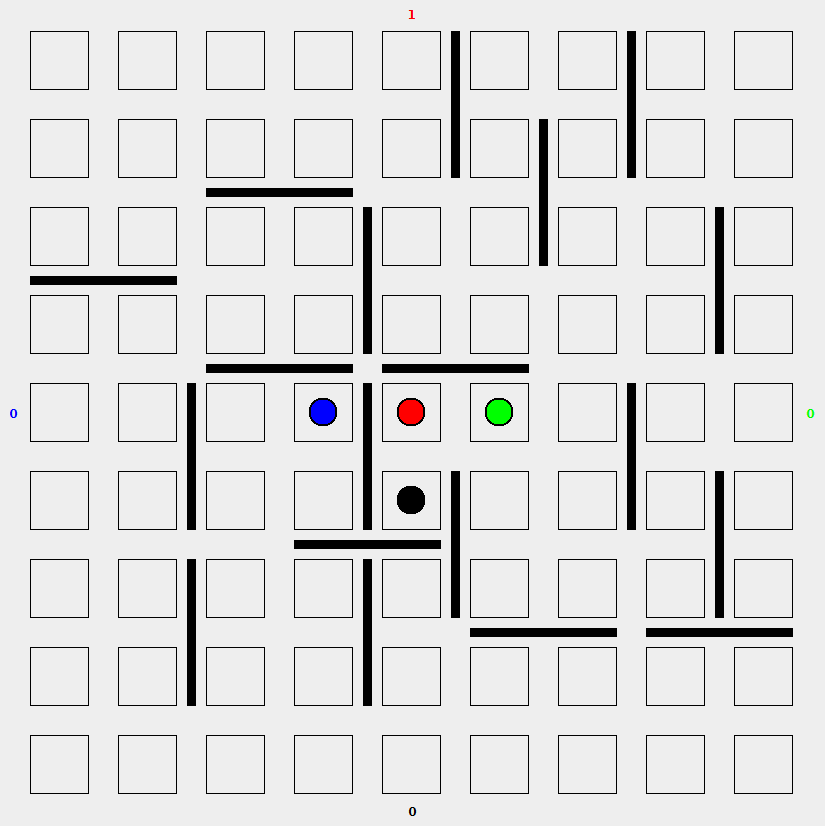
\includegraphics[width=80mm]{no-move.png}
\end{rysunek}

\subsection*{Rozwiązanie problemu}

Zasady nie przewidują sytuacji, w której nie ma legalnych ruchów i żaden gracz nie zwyciężył.
Możliwe wyjścia z tej sytuacji to

\begin{enumerate}
\item \label{loose-turn} odebranie ruchu zablokowanemu graczowi
\item \label{loose-game} uznanie braku możliwych ruchów za porażkę
\item \label{prevent} zakazanie ruchu, który doprowadza do takiej sytuacji
\item \label{solve} dozwolonie dodatkowych ruchów
\end {enumerate}

Jedynym dostępnym kryterium przy dokonaniu wyboru jest tutaj subiektywna jakość rozgrywki, która powinna jak najlepiej przypominać oryginalną grę.
Rozwiązania \ref{loose-turn} i \ref{loose-game} naszym zdaniem nadto zmieniają zasady.
\ref{loose-turn} stwarza możliwość celowego blokowania gracza, aby układać ogrodzenia nie odczuwając kosztu związanego z nie poruszeniem pionka.
\ref{loose-game} jest jeszcze większą ingerencją w dostępne strategie, ponieważ uznając więcej stanów za końcowe pozwala porzucić oryginalne cel rozgrywki, tzn. dotarcie na drugą stronę planszy.
Wadą \ref{prevent} jest mała przejrzystość.
Jeżeli jeden gracz wykonuje ruch, który pozostawia drugiemu tylko jeden możliwy ruch, który w efekcie odbiera trzeciemu wszystkie możliwości, ruch pierwszego gracza powinien być zakazany.
Jest to jednak trudne do spotrzeżenia i gracz pierwszy może nie rozumieć, dlaczego nie może wykonać takiego ruchu.

Wybraliśmy więc rozwiązanie \ref{solve}, poszerzając definicję przeskoczenia pionka przeciwnika.
Zgodnie z nową definicją gracz może przeskoczyć sąsiadujący (i nieodgrodzony) pionek przeciwnika stawiając swój  na dowolnym polu, na który mógłby postawić go przeciwnik, gdyby właśnie wykonywał ruch.
We wcześniej przedstawionym przykładzie, ruch wykonuje gracz czarny.
Gdyby ruch wykonywał gracz czerwony, mógłby przeskoczyć pionek gracza zielonego.
A zatem gracz czerwony również może to zrobić, co daje mu dwa możliwe ruchy do wyboru.

Ponieważ pierwotne zasady gry zapewniają, że każdy gracz ma dostępną przy namniej jedną drogę do celu, nowa definicja przeskoczenia pionka gwarantuje, że zawsze można wykonać ruch pionkiem.

\section{Interfejs bota}

Przed rozwijaniem algorytmów botów należy określić sposób w jaki będzie on udzielał odpowiedzi i ograniczenia, jakie zostaną narzucone.
Musimy tu przede wszystkim wziąć pod uwagę jakość użytkowania aplikacji i ograniczenia urządzeń, na jakich ma być uruchamiana.

Najprostszym interfejsem bota byłaby pojedyncza procedura, która dla zadanego stanu gry zwraca wybrany ruch.
Utrudnia jednak ona właściwe wykorzystanie czasu, jaki bot ma na wybranie ruchu.
Nie ma on możliwości wyboru decyzji jako wydającej się najlepszą w danej chwili i dalszego szukania lepszej.
Jeżeli próbując wykorzystać cały dostępny czas przekroczy go, arbiter przerwie procedurę i w ogóle nie zwróci ona wyniku.

Dlatego jako interfejs bota obraliśmy procedurę nie zwracającą wyniku, która będzie uruchamiana przez aplikację w osobnym procesie na wyznaczony czas, a następnie przerywana.
Podczas działania będzie mogła modyfikować swoją decyzję o wybranym ruchu, będącą obiektem współdzielonym z procesem arbitra aplikacji.

Dla zapewnienia płynności rozgrywki, limit czasu ustalamy na 2 sekundy.
Oczywiście mógłby być konfigurowany przez użytkownika, ale wyszczególnienie pożądanej wartości pomoże w porównywaniu botów i wskazaniu algorytmu, który najlepiej sprawdza się w określonych warunkach.

Ustaliliśmy też przybliżone maksymalne zużycie pamięci na 500 MB, co ma znaczenie zwłaszcza dla algorytmów wykorzystujące tablicę transpozycji, która tym lepiej się sprawdza, im jest większa.
Jednak nasza aplikacja ma działać na współczesnym komputerze osobistym (który ma dziś zwykle 4 GB pamięci), a nie brać udział w potyczkach botów na superkomputerach.

\chapter{Rozwijanie botów}

\chapter{Podsumowanie}

\begin{thebibliography}{98}
\addcontentsline{toc}{chapter}{Bibliografia}

\bibitem[1]{pawlewicz} Jakub Pawlewicz, \textit{Techniki sztucznej inteligencji
    w programach grających}, 2010
\bibitem[2]{sturtevant} Nathan Reed Sturtevant, \textit{Multi-Player Games: Algorithms and Approaches}, 2003
\bibitem[3]{korf} Richard Korf, \textit{Multi-player alpha-beta pruning}, 1991

\end{thebibliography}

\begin{appendices}

\chapter{Kod źródłowy aplikacji}
Na dołączonej płycie znajduje się kod źródłowy.

\end{appendices}

\end{document}


%%% Local Variables:
%%% mode: latex
%%% TeX-master: t
%%% coding: utf-8
%%% End:
